\subsection{DAC-Chip DAC0909} % (fold)
\label{sub:DAC-Chip_DAC0909}

\begin{frame}
    \frametitle{DAC-Chip}
    \framesubtitle{}
    \begin{figure}[H]
        \begin{center}
                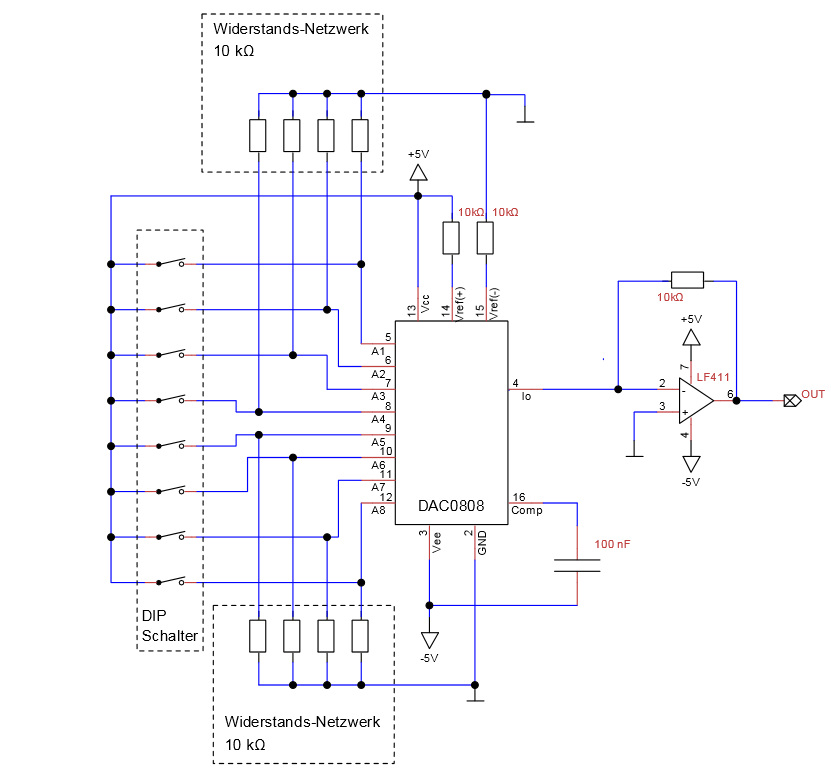
\includegraphics[scale=0.38]{./img/schaltung/dac_0.png}
        \end{center}
    \end{figure}    
\end{frame}

\begin{frame}
    \frametitle{DAC-Chip}
    \framesubtitle{}
    \begin{columns}[c]
        \column{0.5\textwidth}
             \begin{block}{}
                \begin{itemize}
                    \item geringe Ausgangsspannung $\rightarrow$ Operationsverstärker
                \end{itemize}
             \end{block}
        \column{0.5\textwidth}
            \begin{figure}[H]
                \begin{center}
                        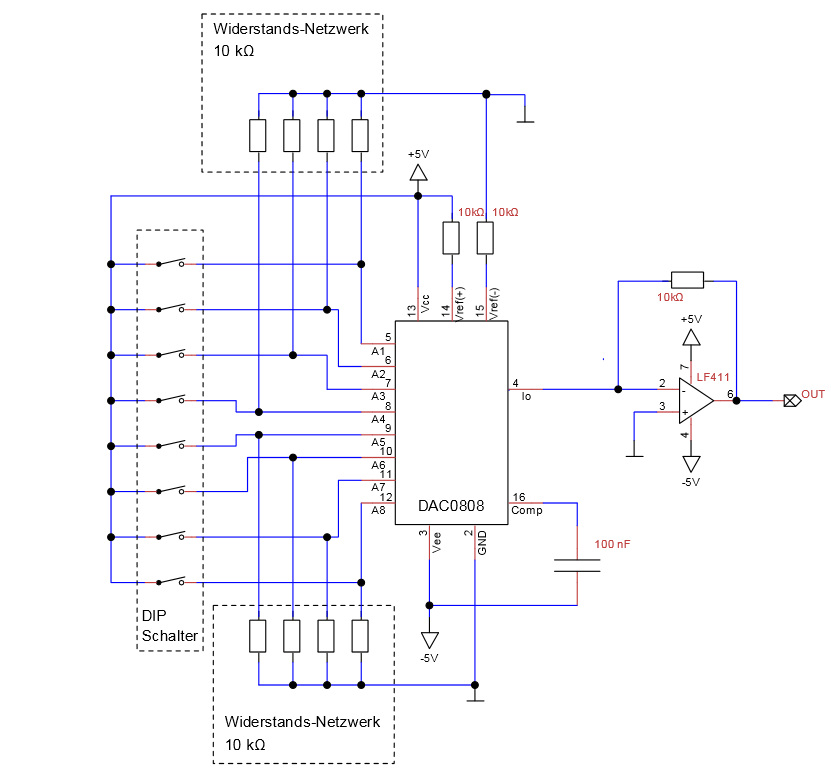
\includegraphics[scale=0.25]{./img/schaltung/dac_0.png}
                \end{center}
            \end{figure}    
    \end{columns}
\end{frame}

\begin{frame}
    \frametitle{Messwerte}
    \framesubtitle{}
    \begin{columns}[c]
        \column{0.6\textwidth}
            \begin{block}{Messung}
                \begin{itemize}
                    \item starke Linearität
                    \item hoher Nullpunktfehler: -$0.496mV$
                    \item Abweichung im hohen Bereich durch Begrenzung der
                    Versorgungsspannung
                \end{itemize}
            \end{block}
        \column{0.4\textwidth}
            \begin{figure}[H]
            \begin{center}
                    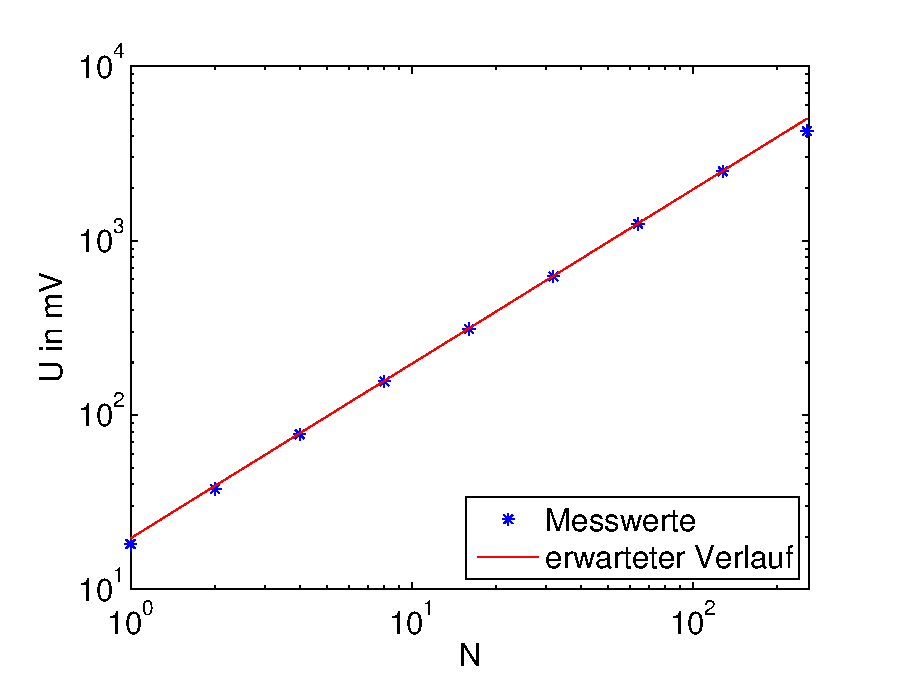
\includegraphics[scale=0.3]{./img/graph/Aufgabe1b.eps}
            \end{center}
            \end{figure}
    \end{columns}
\end{frame}
% subsection DAC-Chip DAC0909 (end)
